%% The LaTeX package tcolorbox - version 4.50 (2021/05/21)
%% tcolorbox-example-poster.tex: a poster example for tcolorbox
%%
%% -------------------------------------------------------------------------------------------
%% Copyright (c) 2006-2021 by Prof. Dr. Dr. Thomas F. Sturm <thomas dot sturm at unibw dot de>
%% -------------------------------------------------------------------------------------------
%%
%% This work may be distributed and/or modified under the
%% conditions of the LaTeX Project Public License, either version 1.3
%% of this license or (at your option) any later version.
%% The latest version of this license is in
%%   http://www.latex-project.org/lppl.txt
%% and version 1.3 or later is part of all distributions of LaTeX
%% version 2005/12/01 or later.
%%
%% This work has the LPPL maintenance status `author-maintained'.
%%
%% This work consists of all files listed in README
%%
% arara: pdflatex: { shell: yes }
% arara: pdflatex: { shell: yes }
\documentclass[12pt]{article}

\usepackage[a3paper,landscape]{geometry}
\usepackage{lipsum}
\usepackage{lmodern}
\usepackage{enumerate}

\usepackage[poster]{tcolorbox}
\tcbuselibrary{minted} % <- replace by \tcbuselibrary{listings}, if minted does not work for you

\pagestyle{empty}

\begin{document}
\begin{tcbposter}[
  coverage = {
      spread,
      interior style={top color=yellow,bottom color=yellow!50!red},
      watermark text={\LaTeX\ Poster},
      watermark color=yellow,
  },
  poster   = {showframe=false,columns=4,rows=5},
  boxes    = {
      enhanced standard jigsaw,sharp corners=downhill,arc=3mm,boxrule=1mm,
      colback=white,opacityback=0.75,colframe=blue,
      title style={left color=black,right color=cyan},
      fonttitle=\bfseries\Large\scshape
   }
]

%----
\posterbox[blankest,interior engine=path,height=3cm,
    halign=center,valign=center,fontupper=\bfseries\large,colupper=red!25!black,
    underlay={
      \node[right,inner sep=0pt,outer sep=0pt] at (frame.west) {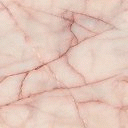
\includegraphics[height=3cm]{pink_marble.png}};
      \node[left,inner sep=0pt,outer sep=0pt] at (frame.east) {
\includegraphics[height=3cm]{crinklepaper.png}};
  },
  ]{name=title,column=1,span=3,below=top}{
  \resizebox{18cm}{!}{\bfseries\Huge My Important Project}\\[3mm]
  Hans.Mustermann@deepthought.university
}

%----
\posterbox[adjusted title=References]{name=references,column=2,span=1.5,above=bottom}{
  \begin{enumerate}[{[1]}]
  \item\label{litA} Important Authors, \textit{Important Title}
  \item\label{litB} More Important Authors, \textit{More Important Title}
  \item\label{litC} Less Important Authors, \textit{Less Important Title}
  \end{enumerate}
}

%----
\posterbox[adjusted title=Process,halign=center]{name=process,column=2,span=2,above=references}{
  
\begin{tikzpicture}[very thick,radius=2cm]
    \begin{scope}
      \path[draw=black,fill=white] (0,0) circle;
      \path[fill=red] (0,0) -- (2,0) arc [start angle=0, end angle=30];
    \end{scope}
    \begin{scope}[xshift=5cm]
      \path[draw=black,fill=white] (0,0) circle;
      \path[fill=red] (0,0) -- (2,0) arc [start angle=0, end angle=70];
    \end{scope}
    \begin{scope}[xshift=10cm]
      \path[draw=black,fill=white] (0,0) circle;
      \path[fill=red] (0,0) -- (2,0) arc [start angle=0, end angle=110];
    \end{scope}
    \begin{scope}[xshift=15cm]
      \path[draw=black,fill=white] (0,0) circle;
      \path[fill=red] (0,0) -- (2,0) arc [start angle=0, end angle=240];
    \end{scope}
  \end{tikzpicture}
}

%----
\posterbox[adjusted title=Project Description]{name=project,
    sequence=1 between title and bottom then 2 between title and process}{
  See [\ref{litA}]: \lipsum[1]
  \begin{center}
  \tikz \draw[thick,rounded corners=8pt]
    (0,0)--(0,2)--(1,3.25)--(2,2)--(2,0)--(0,2)--(2,2)--(0,0)--(2,0);
  \quad by [\ref{litB}]
  \end{center}
  \lipsum[2-3]\par
  See [\ref{litC}]:
  \lipsum[4]
  \begin{center}
  \tikz \shadedraw [left color=red,right color=blue]
    (0,0) rectangle (2,2);
  \end{center}
  That's all.
}

%----
\posterbox[adjusted title=Central Picture,
  interior style={fill overzoom image=blueshade.png}]
  {name=picture,column=3,between=title and process}{}

%----
\begin{posterboxenv}[adjusted title=Core Algorithm,leftupper=0pt,rightupper=0pt]
  {name=algorithm,column=4,between=top and references}
\begin{tcblisting}{blankest,listing only}

\begin{tikzpicture}[very thick,radius=2cm]
  \begin{scope}
    \path[draw=black,fill=white] (0,0) circle;
    \path[fill=red] (0,0) -- (2,0)
      arc [start angle=0, end angle=30];
  \end{scope}
  \begin{scope}[xshift=5cm]
    \path[draw=black,fill=white] (0,0) circle;
    \path[fill=red] (0,0) -- (2,0)
      arc [start angle=0, end angle=70];
  \end{scope}
  \begin{scope}[xshift=10cm]
    \path[draw=black,fill=white] (0,0) circle;
    \path[fill=red] (0,0) -- (2,0)
      arc [start angle=0, end angle=110];
  \end{scope}
  \begin{scope}[xshift=15cm]
    \path[draw=black,fill=white] (0,0) circle;
    \path[fill=red] (0,0) -- (2,0)
      arc [start angle=0, end angle=240];
  \end{scope}
\end{tikzpicture}

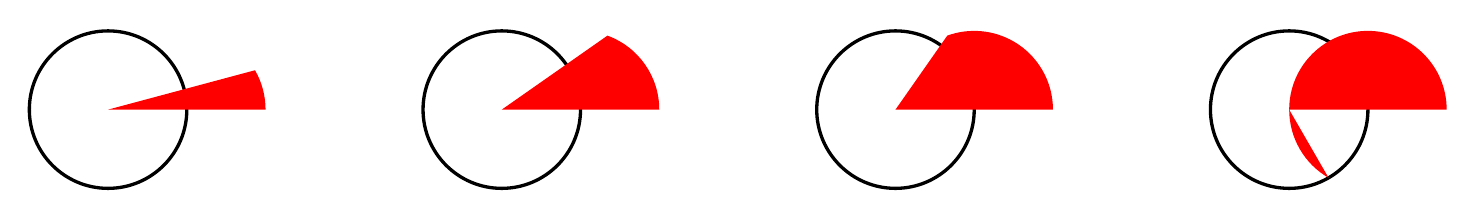
\begin{tikzpicture}[very thick,radius=1cm]
  \begin{scope}
    \path[draw=black,fill=white] (0,0) circle;
    \path[fill=red] (0,0) -- (2,0)
      arc [start angle=0, end angle=30];
  \end{scope}
  \begin{scope}[xshift=5cm]
    \path[draw=black,fill=white] (0,0) circle;
    \path[fill=red] (0,0) -- (2,0)
      arc [start angle=0, end angle=70];
  \end{scope}
  \begin{scope}[xshift=10cm]
    \path[draw=black,fill=white] (0,0) circle;
    \path[fill=red] (0,0) -- (2,0)
      arc [start angle=0, end angle=110];
  \end{scope}
  \begin{scope}[xshift=15cm]
    \path[draw=black,fill=white] (0,0) circle;
    \path[fill=red] (0,0) -- (2,0)
      arc [start angle=0, end angle=240];
  \end{scope}
\end{tikzpicture}
\end{tcblisting}
\end{posterboxenv}

%----
\posterbox[adjusted title=Contact,fit,fit basedim=12pt]
    {name=contact,column*=4,span=1.5,between=process and bottom}{
  \lipsum[2]
}

\end{tcbposter}
\end{document}
